\subsection{Время рендеринга}

Результаты измерения времени рендеринга изображены на \ref{fig:perfomance}.

\begin{figure}[h!]
    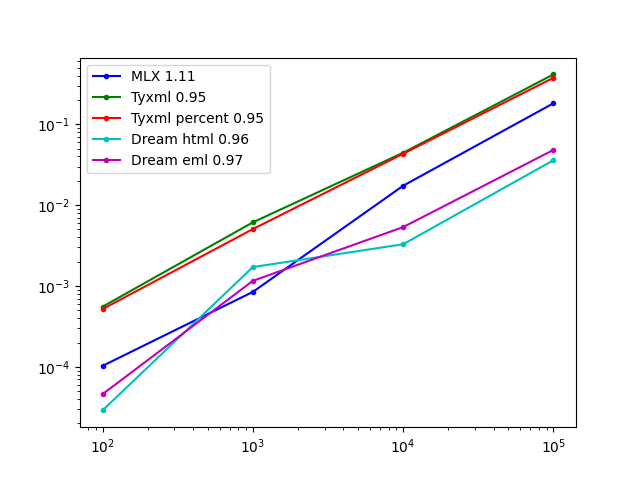
\includegraphics[width=\textwidth]{perfomance.png}
    \caption{Сравнение производительности шаблонизаторов. График построен с помощью пакета matplotlib. Числа в легенде соответствуют аппроксиммированному углу наклона прямых. Масштаб выбран логарифмическим для удобства. Дополнительные детали анализа можно также найти в \ref{apx:tyxml_performance}}
    \label{fig:perfomance}
\end{figure}

\begin{figure}[h!]
    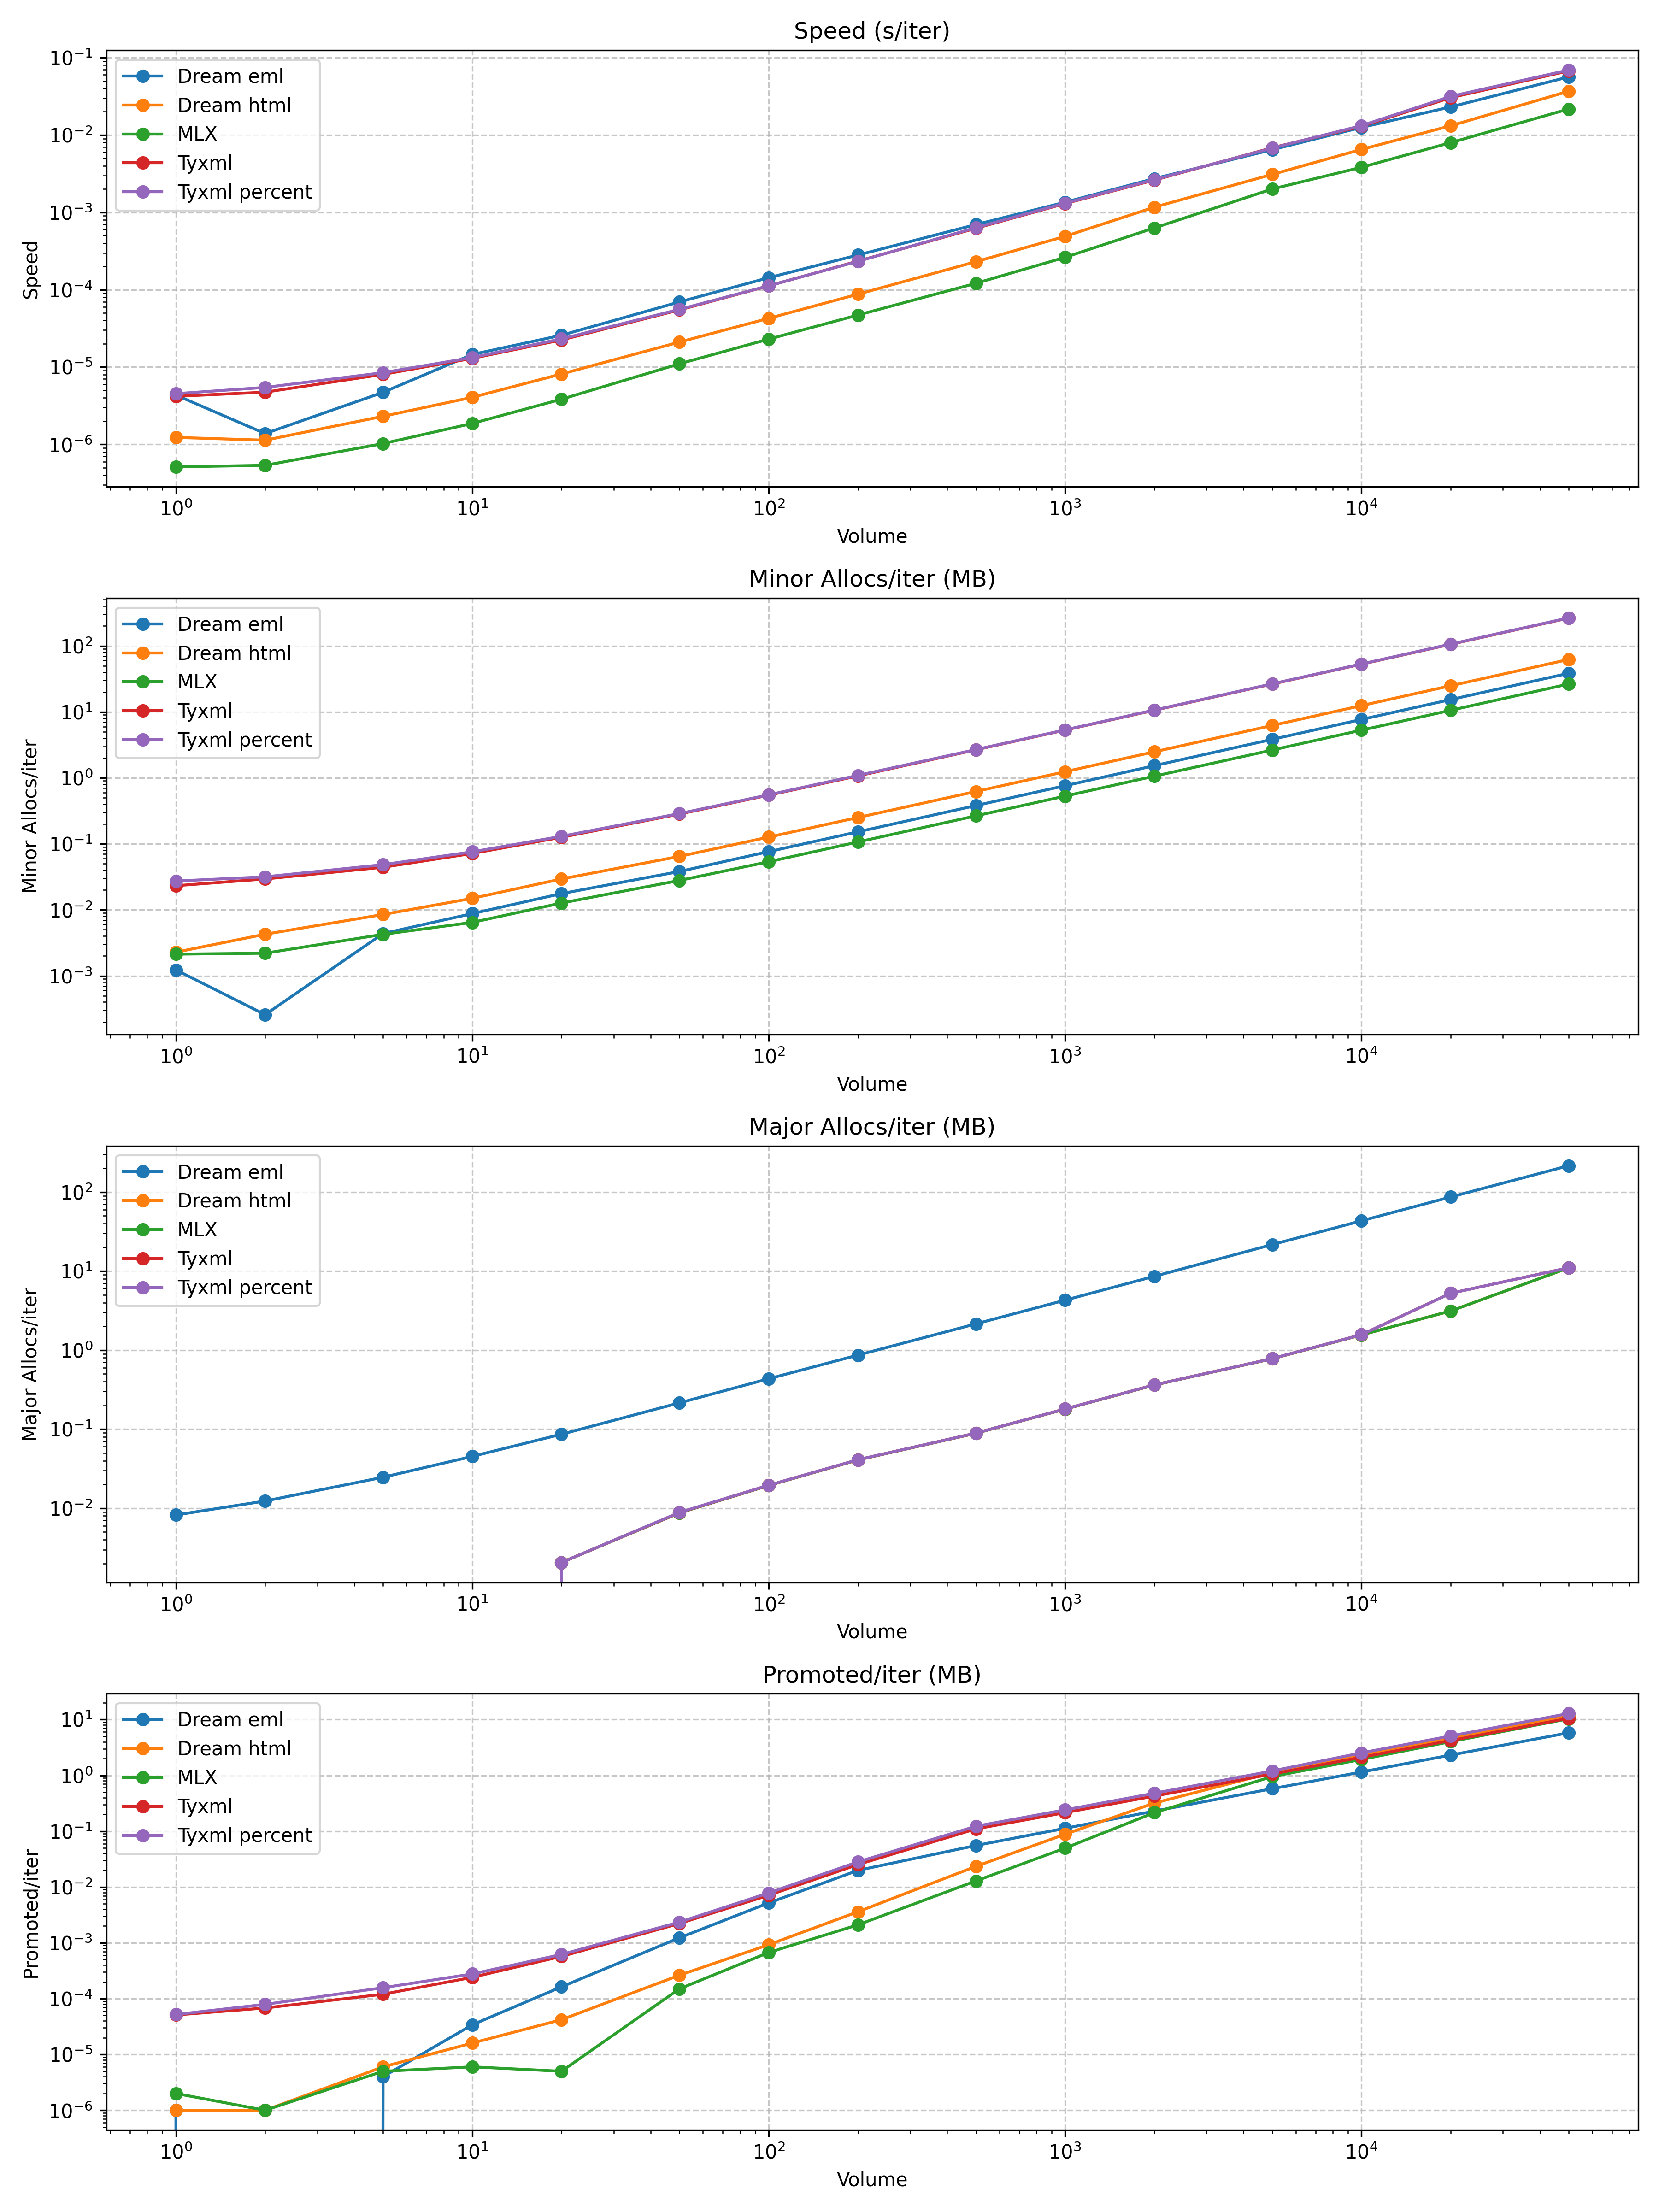
\includegraphics[width=\textwidth]{benchmark_results.png}
    \caption{}
    \label{fig:bench-performance}
\end{figure}

Как видно из графика\ref{fig:bench-performance}, EML выделяет значительно больше долгосрочной памяти чем остальные фреймворки.
Кроме того, он медленнее работает.

TyXML показал также неутешительные результаты, работая медленнее MLX и Dream HTML.

Самым производительным с точки зрения и аллокаций и скорости оказался MLX.


